\documentclass[journal, 12pt]{IEEEtran}

% *** CITATION PACKAGES ***
%
%\usepackage{cite}https://www.overleaf.com/project/5d8e32cf8b64620001d24060
\usepackage{capt-of}%%To get the caption
\usepackage{gensymb}
\usepackage{graphicx} %package to manage images
\graphicspath{ {./images/} }
\usepackage{wrapfig}

\usepackage{amsmath}
\usepackage{amssymb}
\usepackage{hyperref}
\usepackage{lipsum}

\usepackage[style=ieee]{biblatex}
\DeclareLanguageMapping{english}{english-apa}
\addbibresource{references.bib}
\usepackage[justification=centering]{caption}

\usepackage{setspace}

\usepackage{hhline}


\usepackage{changepage} 

\usepackage{booktabs}
\usepackage{xcolor}

\usepackage{makecell}
\usepackage{graphicx,subcaption}
\usepackage{listings}
\renewcommand\theadfont{}
\DeclareMathOperator{\EX}{\mathbb{E}}% expected value


\usepackage{multicol} 

\raggedbottom

\renewcommand{\ttdefault}{txtt}
\lstset{
  language=bash,
  basicstyle=\ttfamily,
  numbers=left,
stepnumber=1,
showstringspaces=false,
tabsize=1,
breaklines=true,
breakatwhitespace=false,
}

\linespread{1.15} 

\begin{document}


\pagenumbering{gobble}
%\clearpage\mbox{} % adds and empty page
%\clearpage
\pagenumbering{arabic}
\setcounter{page}{1}

\title{\Large{Flyway: Crowdedness Detection and Prediction Based on Surrounding Wi-Fi Signals and Reccurent Neural Networks}}

\author{ ENGR-UH 4560 Machine Learning, Fall 2019\\
\medskip
Nishant Aswani,~\IEEEmembership{nsa325@nyu.edu} \;\;
Barkin Simsek,~\IEEEmembership{bs3528@nyu.edu}}% <-this % stops a space


% The paper headers
\markboth{Aswani, Simsek ENGR-UH 4560 Machine Learning, Fall 2019}%
{}

% make the title area
\maketitle

% As a general rule, do not put math, special symbols or citations
% in the abstract or keywords.
% \begin{abstract}


% \end{abstract}

%%%%%%%%%%%%%%%%%%
%% Introduction %%
%%%%%%%%%%%%%%%%%%
\section{Introduction}
\subsection{Motivation}
\IEEEPARstart{P}\lowercase{redicting} traffic is one of the most common timeseries forecasting problems available for tackling. When placed in the context of smart cities, the problem is motivated by the question of "how to enable users to make smarter choices when using transportation networks" \cite{lv2014traffic}. However, this can be broadened to include how smart choices are made for using infrastructure and public spaces in general. \\

\noindent Given that our campus has multiple open spaces for students to study and/or relax, we want to be able to forecast the crowdedness that occurs in these spaces. When combined with an interface to visualize the forecasts and historical data, this can be used as a powerful decision making tool.

\subsection{Problem Statement}
\noindent It is a known fact among the NYUAD community that NYUAD’s class size is growing rapidly as shown in Figure \ref{fig:student_bar} while the number of available physical space stays the same. Some students struggle with finding silent and not crowded places to study alone while some students struggle with finding an unoccupied room to party with their friends. Unfortunately, this problem only gets worse as the number of students increase on the campus. This problem is not only limited to students as well. Similarly, it is known that faculty struggle with finding places to eat during the launch break without waiting in a very long time that wastes time. Thus, we need a way to control crowds at NYUAD and redirect crowds to certain places when needed.

\begingroup
    \center
    \medskip
    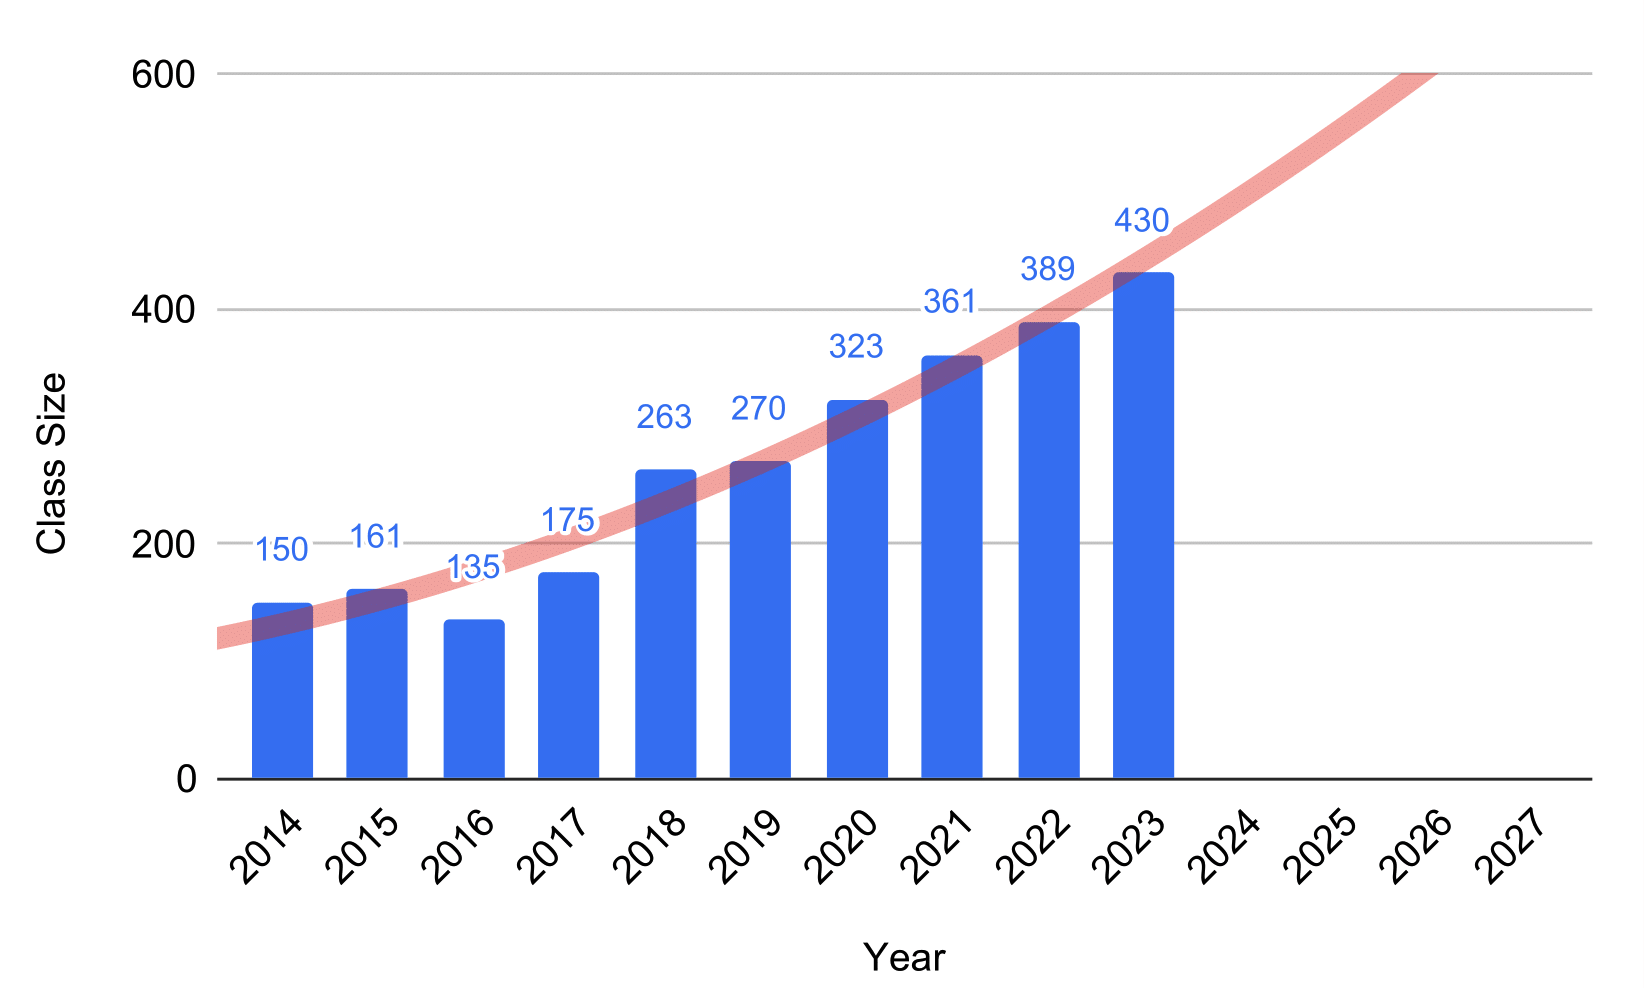
\includegraphics[width=\columnwidth]{report/final_report/images/student_bar.png}
    \captionof{figure}{Student population per class at NYUAD over years [\href{https://nyuad.nyu.edu/}{Data Source}]}
    \label{fig:student_bar}
    \medskip
\endgroup

\noindent One way to tackle this problem is creating a platform for community members to monitor crowdedness around the campus and providing accurate predictions towards the future. Machine learning is a great tool for achieving this since we can model the crowdedness around the campus as a time-series data. There are good machine learning tools to solve this time-series forecasting problem and distribute crowds evenly around the campus.\\

\noindent In order to gather a sense of crowdedness in a room, we determined that registering the device addresses along with packet transfers would be a robust method involving little overhead. Students almost always carry their laptops and mobile devices with them as they move around on campus. \\

\noindent Hence, our project aims to forecast the crowdedness of a location using a combination of the number of unique Media Access Control (MAC) addresses and the number of wireless data packages sent within a given hour coupled with a powerful neural network. 

\subsection{High Level Overview \& Formulation}
\noindent As an high level overview, we can state that our project captures surrounding WiFi signals as a time-series data as input to the system, and applies machine learning models to predict the future crowdedness of places around the campus. Finally, it provides a user friendly application interface for presenting the produced forecasts as the output of the system.

\begingroup
    \centering
    \medskip
    %width=\columnwidth
    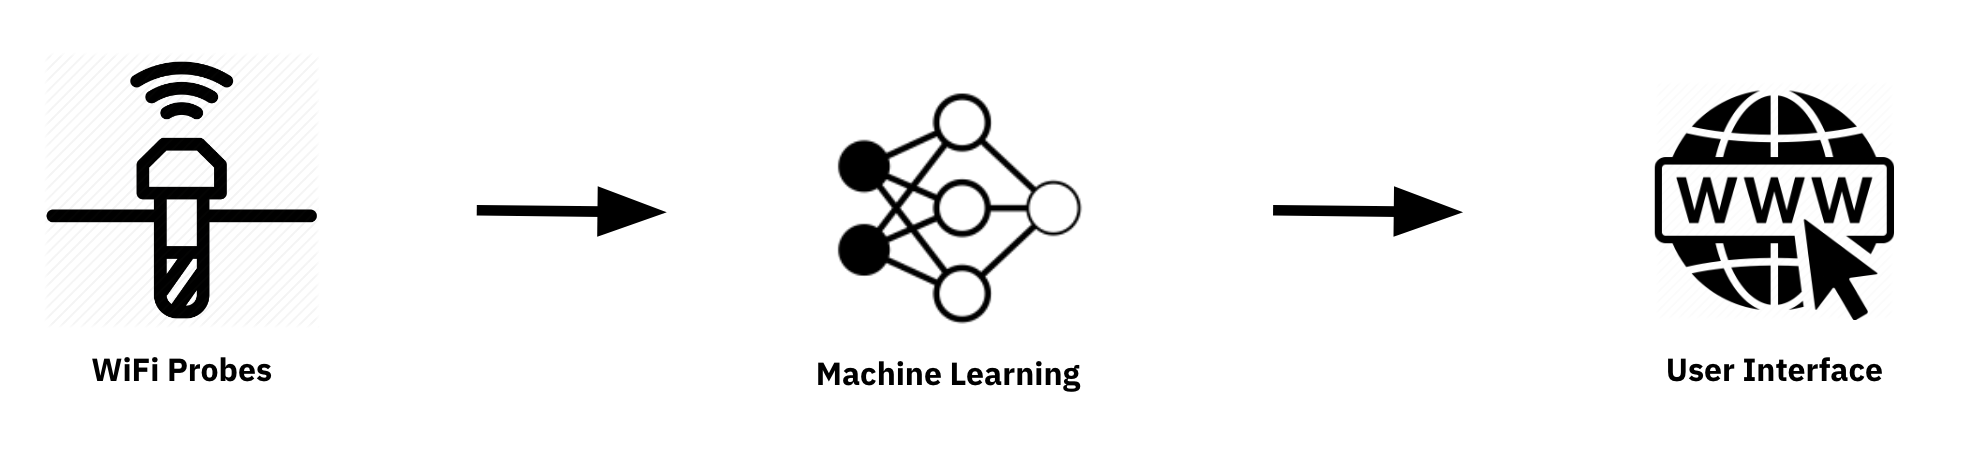
\includegraphics[width=\columnwidth]{./images/formulation.png}
    \captionof{figure}{High level overview of the project}
    \label{fig:formulation}
    \medskip
\endgroup

%%%%%%%%
% NOTE %
%%%%%%%%
% include info about how we gather the data, why we gather the data that way, and why we get that specific data or those features

\section{Existing Body of Work}
\subsection{Past Projects}
\noindent One of the inspirations of this project was the Waitz application developed by students at University of California San Diego (UCSD) \cite{waitz}. They used Raspberry Pis, loaded with network monitoring firmware and placed at various locations around their campus, to approximate the number of students within a given area. They did so by logging the Bluetooth and MAC addresses of devices within range of the network-sniffing Raspberry Pi's. This data is then presented to users in the form of a mobile app, allowing them to make decisions based on live crowdedness measurements.\\

\noindent However, their application is relatively simple as they did not use their data to forecast the crowdedness of locations or make any predictions. Instead, it seems that they focused more on data collection and providing a live metric. Drawing inspiration, we sought implement a similar tool for our campus, hoping to further their idea and discover if there are any time-series patterns we can exploit to provide worthwhile forecasts.\\

\noindent Another practical application we have encountered was Facebook's Prophet tool. This tool is designed as a more generic infrastructure maintenance and planning tool rather than predicting crowdedness in Facebook's facilities. Their tool tries to capture cyclic human behaviour and daily routines to report anything that doesn't go as planned at Facebook facilities. For example, if most of the employees use a certain car park all the time and if employees stop using that car park, the system detects the anomaly in that part of the facility and reports to managers. Similarly, they also use this tool for planning to build new facilities if a facility is not capable of meeting the demand. Facebook's Prophet tool was another inspiration source for us since it proved that the trends and cycles in a time-series data can be used for a more accurate forecasting.

\begingroup
    \centering
    \medskip
    %width=\columnwidth
    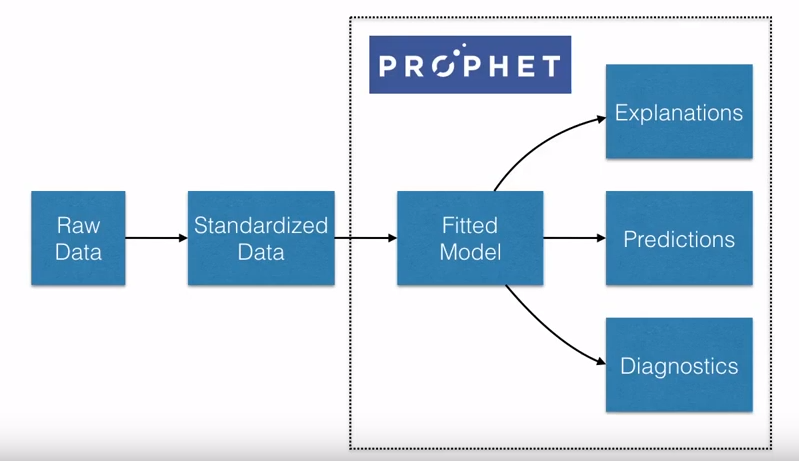
\includegraphics[width=\columnwidth]{./images/prophet.png}
    \captionof{figure}{Facebook’s Prophet's workflow for forecasting at scale}
    \label{fig:facebook}
\endgroup

\subsection{Literature}
\noindent Unsurprisingly, there have been several attempts at using machine learning to determine crowdedness. We found that some of the published work refers to this field as "occupancy prediction" using "Wi-Fi probing"\cite{wang2018occupancy}. Specifically, the work published by Wang et. al. discovered some reassuring key characteristics regarding their dataset in their occupancy prediction project. They realized their collected data had a "time-series characteristics" \cite{wang2018occupancy}, adding weight to our hypothesis that occupancy is relative to time of day, as well as the idea that past data can feasibly predict future data. While this may be trivial to the overall project, it was a source of confidence for us, as it implied we could successfully build a reasonably performing model. \\

\noindent The researchers implemented a "Markov-based feedback Recurrent Neural Networks (M-FRNN)" \cite{wang2018occupancy} model to predict occupancy. They described their neural network as having 3 layers, with the input layer accepting a vector of hashed MAC addresses, at a given time t. Moreover, they acknowledged that their raw data had fluctuations and noise that could potentially "deteriorate the prediction accuracy" \cite{wang2018occupancy}. To avoid this, they added a feature layer between the input and hidden layer, which calculates the "transfer probabilities" for every given MAC address at time t\cite{wang2018occupancy}. They describe their matrix of transfer probabilities (TPMI) as: 

\begin{gather}
 TPMI
 =
  \begin{bmatrix}
   X_{k}^{i-o} & X_{k}^{i-i}\\
   X_{k}^{o-o} & X_{k}^{o-i}\\
   \end{bmatrix}
\end{gather}

\noindent where each element is a conditional probability. For example, $X_{k}^{i-o}$ refers to the conditional probability:

\begin{equation}
    \begin{split}
        X_{k}^{i-o} = \frac{\sum{\text{from in to out}}}{\sum{\text{from in to in}} + \sum{\text{from in to out}}}
    \end{split}
    \label{eq:}
\end{equation}

\medskip
\noindent They then use the quantities $X_{k}^{o-i}$ and $X_{k}^{i-i}$ as an updated input for their hidden layer. The output of the hidden layer is sent to the Context layer (serving as a short-term memory), which then feeds back into the hidden layer at each run of the network \cite{wang2018occupancy}. Their error function was simply a square of the actual occupancy subtracted from the predicted occupancy\cite{wang2018occupancy}.\\

Studying this paper was crucial, as it provided us with a model and understanding on how to build a machine learning solution. It also helped us better understand the different roles the various models play in certain problems. For example, recurrent neural networks are the primary drivers in a time-series forecasting problem.

\subsection{Constraints}

\noindent The work done in Wang. et. al. was a source of inspiration for us to explore machine learning models used in time-series forecasting. However, the specifics of their approach did not align with our project as they had a greater number of validational resources at hand. For example, Figure \ref{fig:wang_infra} shows that the research group used CO$_2$ meters as a second predictor as well as a camera, allowing them to directly work with the number of people in a given space.\\

\begingroup
    \centering
    \medskip
    %width=\columnwidth
    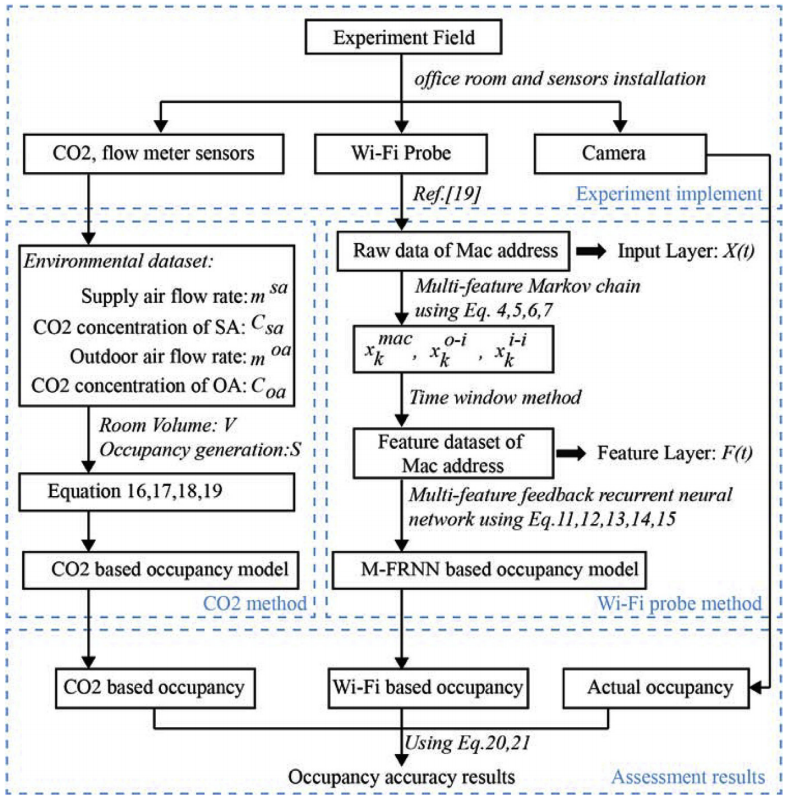
\includegraphics[width=\columnwidth]{./images/wang_model.png}
    \captionof{figure}{The infrastructure used in Wang. et. al's work \cite{wang2018occupancy}}
    \label{fig:wang_infra}
    \medskip
\endgroup


\noindent Due to the time constraints and not having access to enough resources within the time frame of the project, we only used the WiFi probe for collecting the wireless network traffic around the campus. Instead we wanted to maximize what we can get out of collecting MAC addresses without having additional validational data. We decided to focus on unique MAC addresses and the number of data packets sent over the air, which can both be collected with a WiFi probe. Therefore, we used the WiFi branch shown in Figure \ref{fig:wang_infra} as our foundation and we have developed many additional features on top of the foundation, which was inspired by Wang. et. al's work.





\section{Methodology}
\noindent The methodology for realizing this project has 4 main steps: data collection, data processing, data analysis, and a user interface. Having looked at previous work, we confidently determined that each of these steps was feasible, given correct hardware and a careful machine learning implementation.

\subsection{Data Collection: Experimental Setup}
\noindent Data collection was the first step in our process, achieved by deploying the ARM-based Raspberry Pi (RPi) Zero computers, given their built-in Bluetooth and Wi-Fi chips. Specifically, we discovered that it was important that the Wi-Fi chip support "monitoring" mode in order to passively monitor wireless traffic, which is the case with RPi Zero. A computer was set-up for data collection in New York University Abu Dhabi's Engineering Design Studio (EDS). 

\begingroup
    \center
    \medskip
    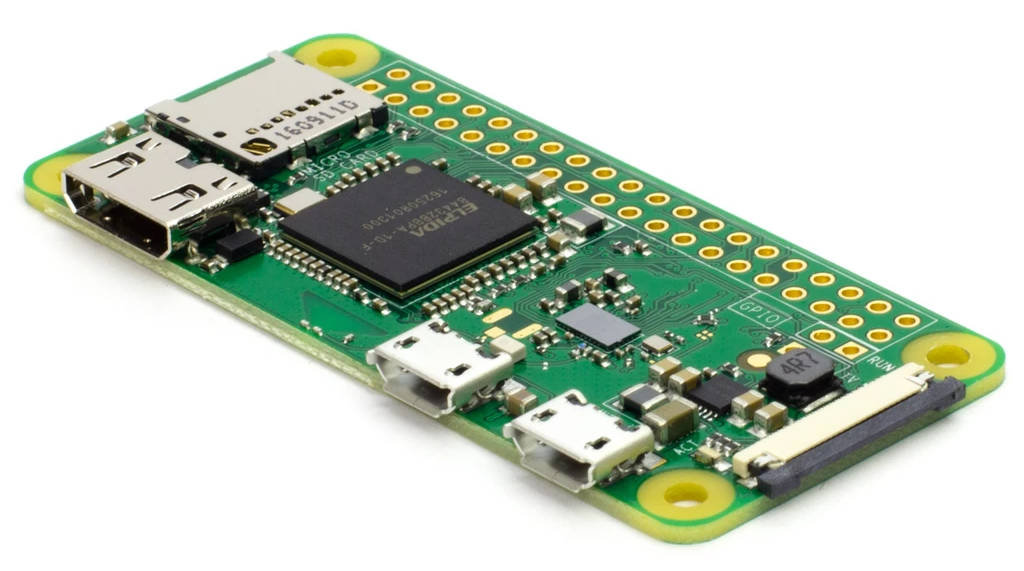
\includegraphics[width=0.6\columnwidth]{report/interim_report/images/raspi.png}
    \captionof{figure}{Raspberry Pi Zero used for data collection}
    \label{fig:raspi}
    \medskip
\endgroup

\noindent Running the Linux operating system, the RPi Zero computer required very little in terms of set-up. The Linux operating system natively supports the \texttt{dumpcap} tool, which was used to collect metadata regarding the packages being sent within range of the device \cite{dumpcap}. 

\begingroup
    \center
    \medskip
    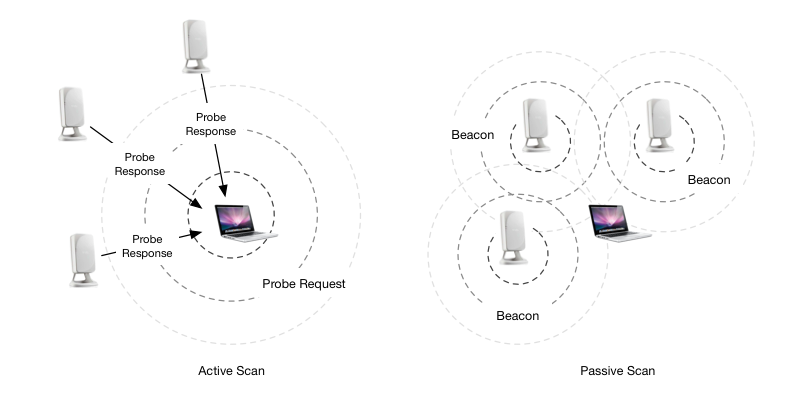
\includegraphics[width=\columnwidth]{report/interim_report/images/scan.png}
    \captionof{figure}{The difference between the active and passive scanning is demonstrated \cite{scanning_image}}
    \label{fig:scannig_types}
    \medskip
\endgroup

\noindent Dumpcap is also capable of recording in both active and passive scanning modes that we can collect an extensive amount of data about the devices in the surrounding space. When in monitoring mode, a Wi-Fi chip is not capable of collecting private data since Wi-Fi traffic between devices and routers are encrypted. That being said, monitoring traffic provides various metadata regarding transferred packages, such as the source and destination. Such non-private information is sufficient, as it can be used to determine number of unique devices as well as extrapolate the network activity in a given time slice. The following are the data fields that can be collected while monitoring Wi-Fi signals in the monitoring mode:
\begin{itemize}
    \item \texttt{frame.number}
    \item \texttt{frame.time}
    \item \texttt{wlan.addr}
    \item \texttt{wlan.ta}
    \item \texttt{wlan.ra}
    \item \texttt{wlan.sa}
    \item \texttt{wlan.da}
    \item \texttt{wlan.bssid}
    \item \texttt{wlan.fc.type}
    \item \texttt{wlan.fc.type\_subtype}
    \item \texttt{radiotap.channel.freq}
    \item \texttt{radiotap.datarate}
    \item \texttt{radiotap.dbm\_antsignal}
\end{itemize}
\medskip
\noindent Here, \texttt{frame.number} and \texttt{frame.time} are fields that contain date time information about the data package. These fields are useful for creating a time-series dataset out of the collected network traffic. The fields that start with \texttt{wlan} relay information regarding the source and destination of the data packets, given in the form of MAC addresses per packet. This information is useful for counting and classifying the number of devices nearby, since MAC addreses are unique to each device. Finally, fields that begin with \texttt{radiotap} have information regarding the signal strength, wireless frequency, and the data rate that channel support. These fields are useful for understanding the proximity of these Wi-Fi device and making decisions about whether to include or not to include certain devices within the dataset.

\subsection{Data Collection: Sniffing WiFi Traffic}
\noindent For demonstrating the functionality of the proposed system, a Raspberry Pi was setup in the Engineering Design Studio (EDS). The Raspberry Pi collected more than a million data packages over two weeks. Collected data was originally captured inside a pcap file format, which is not competible with the machine learning models. Thus, collected data was exported into CSV file format using a Python script and later the CSV file imported into a Pandas dataframe inside the Jupyter Notebook. The Pandas dataframe preview of the collected data can be seen in Figure \ref{fig:pandas}.

\begingroup
    \center
    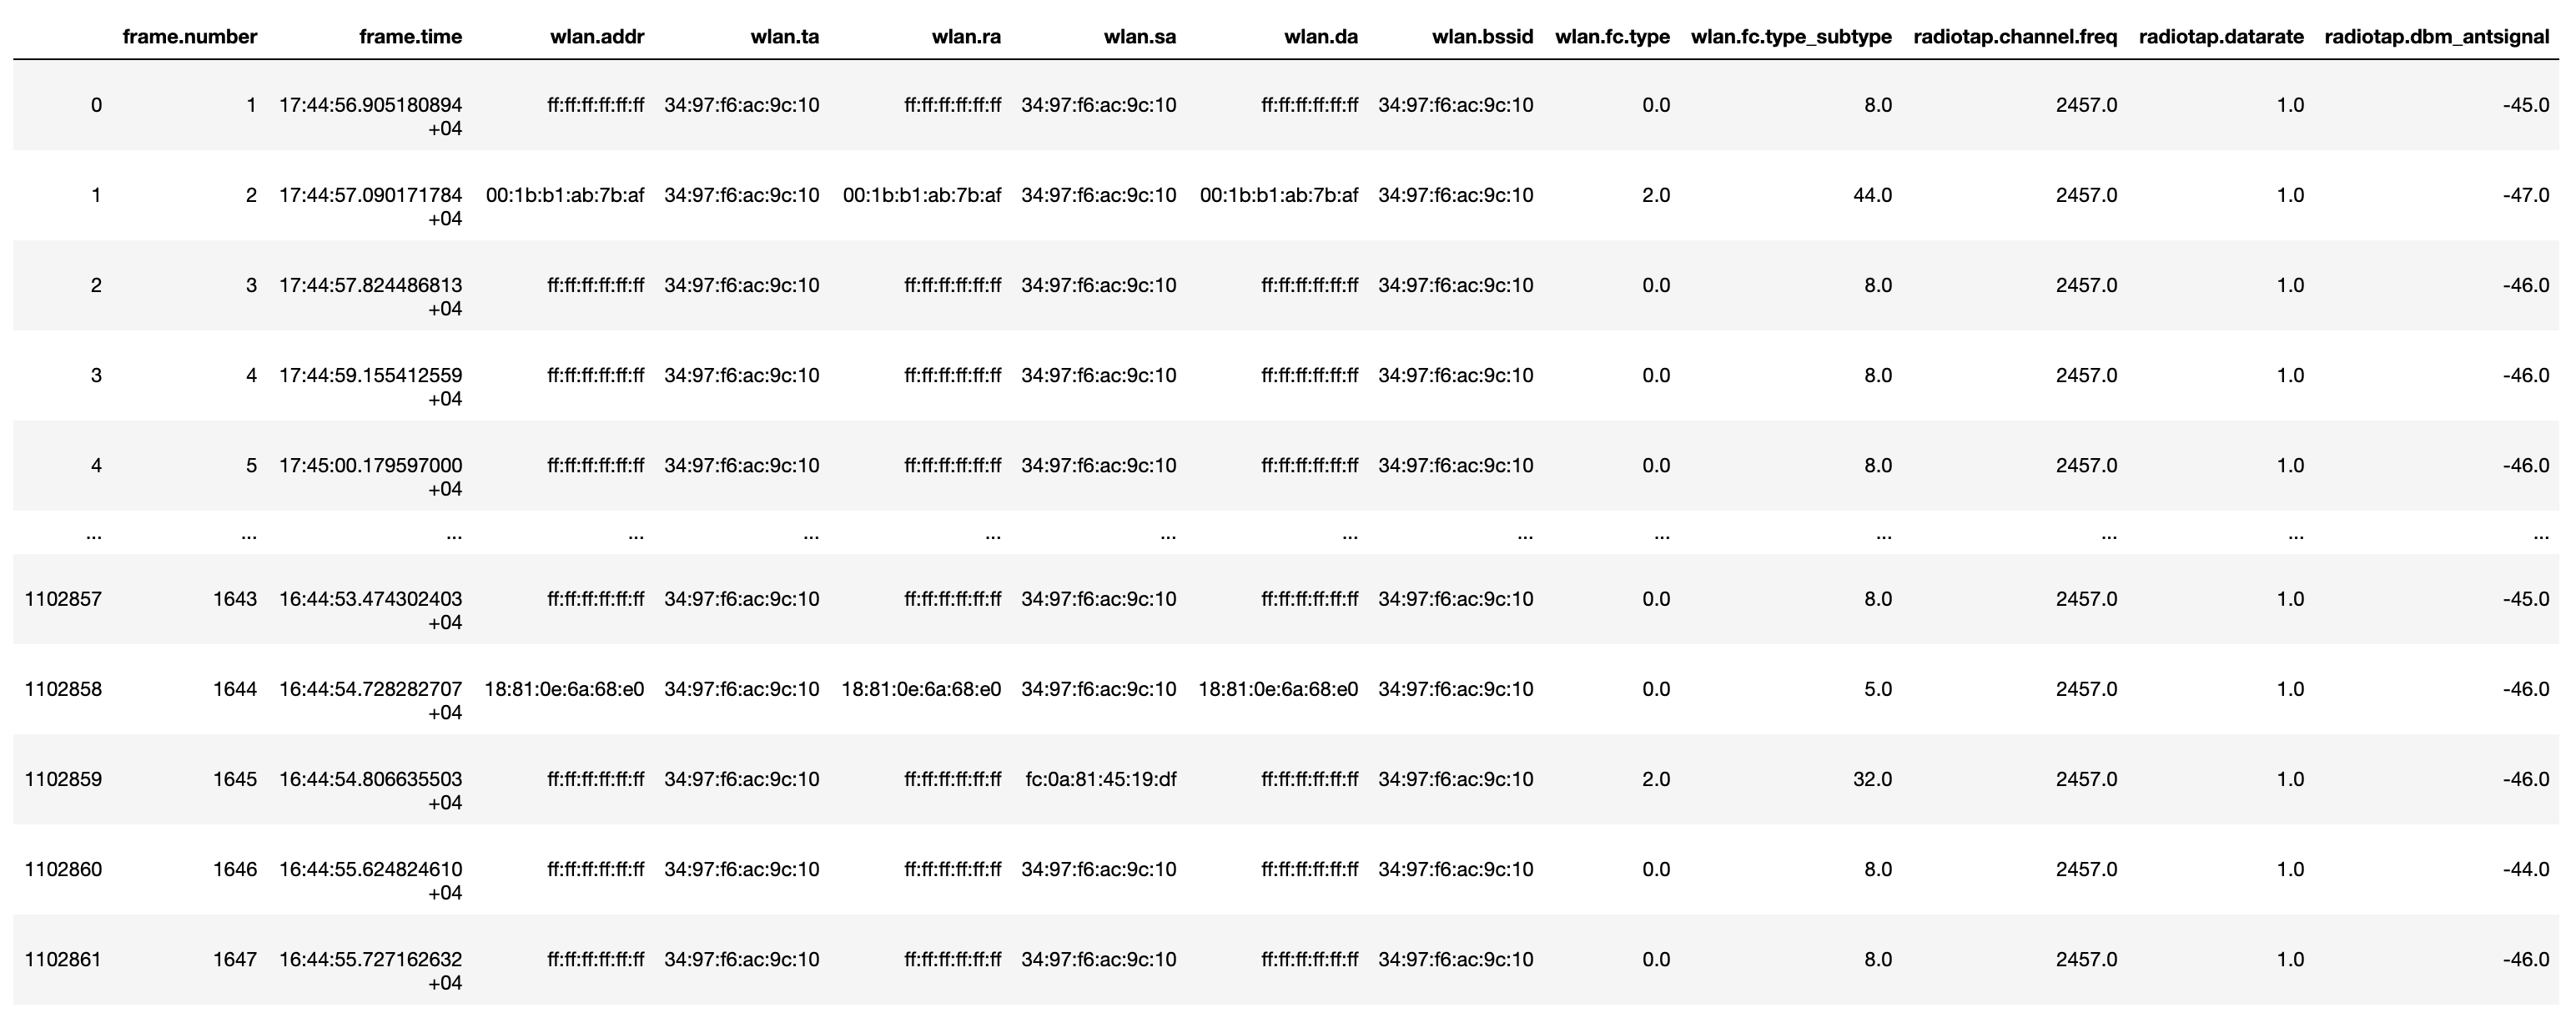
\includegraphics[width=\columnwidth]{report/interim_report/images/pandas.png}
    \captionof{figure}{Preview of the Pandas dataframe created with the collected network traffic}
    \label{fig:pandas}
\endgroup

\subsection{Data Processing: Data Cleaning} 
\noindent As is standard practice, the collected data was cleaned to remove invalid and empty values. Given that the EDS hosts various other non-user devices, such as RPis from other projects, we subtracted all of these devices from our dataset. Moreover, we removed other "loud" devices, such as the router and nearby static devices that were not registered on the EDS network. These operations proved to be significant and severely changed the shape of our package count graph. Please see Appendix A for the large format screen shots of the dataset before and after the data cleaning.

%  Later, the MAC addresses collected under the \texttt{wlan} fields should be validated using the MAC address rules defined by the Institute of Electrical and Electronics Engineers (IEEE). Later, the MAC addresses should be converted into their decimal representations. Normally, MAC addresses are concatenated hexadecimal values and they are stored as strings since they contain letters inside them. However, we cannot use strings with machine learning algorithms and we need to get the decimal representation of each mac address to use the machine learning algorithms for analysing data in the next step. In addition to this, storing MAC addresses of devices might violate privacy of individuals. Therefore, MAC addresses can be hashed using hashing algorithms like MD5 to anonymized the data collected. Hash algorithms generate a hexadecimal value based on the input. Therefore, using a hashing algorithm is also useful for converting the non-numerical MAC address data into a numerical value as shown in the example below:

% \medskip
% \begin{lstlisting}[language=python, numbers=none, mathescape]
% import hashlib
% mac = "34:97:f6:ac:9c:10"
% obj = hashlib.md5(mac.encode())
% hash_hex = obj.hexdigest()
% hash_dec = int(hash_hex, 16)
% print(hash_dec)
% \end{lstlisting}
% \medskip
% \noindent The output of the operation above would be $239801908384185789790176606167296229703$ and it is not reversible, which means that the original MAC address is no longer stored. That being said the hashing function will generate the same number if same exact MAC address is given and this is helpful for finding and avoiding duplicates in the data while preserving the privacy. Thus, the data processing step is crucial for having high quality data for training. \\

\subsection{Data Processing: Data Engineering \& Consideration} 
\label{section:data_engineering}

\noindent As will be justified in Section \ref{section:model_design}, the overarching machine learning model was designed to be modular, with multiple models underneath. Hence, each model was separately trained and required its own dataset to be trained on.\\

\noindent The first model aimed to forecast the number of packages sent at hour $t$, given package count from $t-3$ up to $t-1$, as well as the hour of the day (HoD) and day of the week (DoW). To avoid the model from implicitly assuming ordinal relationships within the data, the HoD and DoW categories were one-hot encoded. While it is generally understood that standardizing or normalizing continuous data, such as package count, improves model performance, it was discovered that this deteriorated the performance in our case.\\ 

\noindent The next model performed a similar task, forecasting the number of unique MAC addresses, at hour t, given package count from $t-3$ up to $t-2$. For this model, it was decided to simply provide the count from previous time steps without additional categorical data to evaluate whether it was necessary. The model performance shows that information regarding the HoD and DoW was unnecessary to providing a good forecast. \\

\noindent Finally, a third dataset was formulated to predict the crowdedness, given the package count and the number of unique MAC addresses. This raised the challenge of providing a more concrete definition of what crowdedness was. 

\begingroup
    \center
    \medskip
    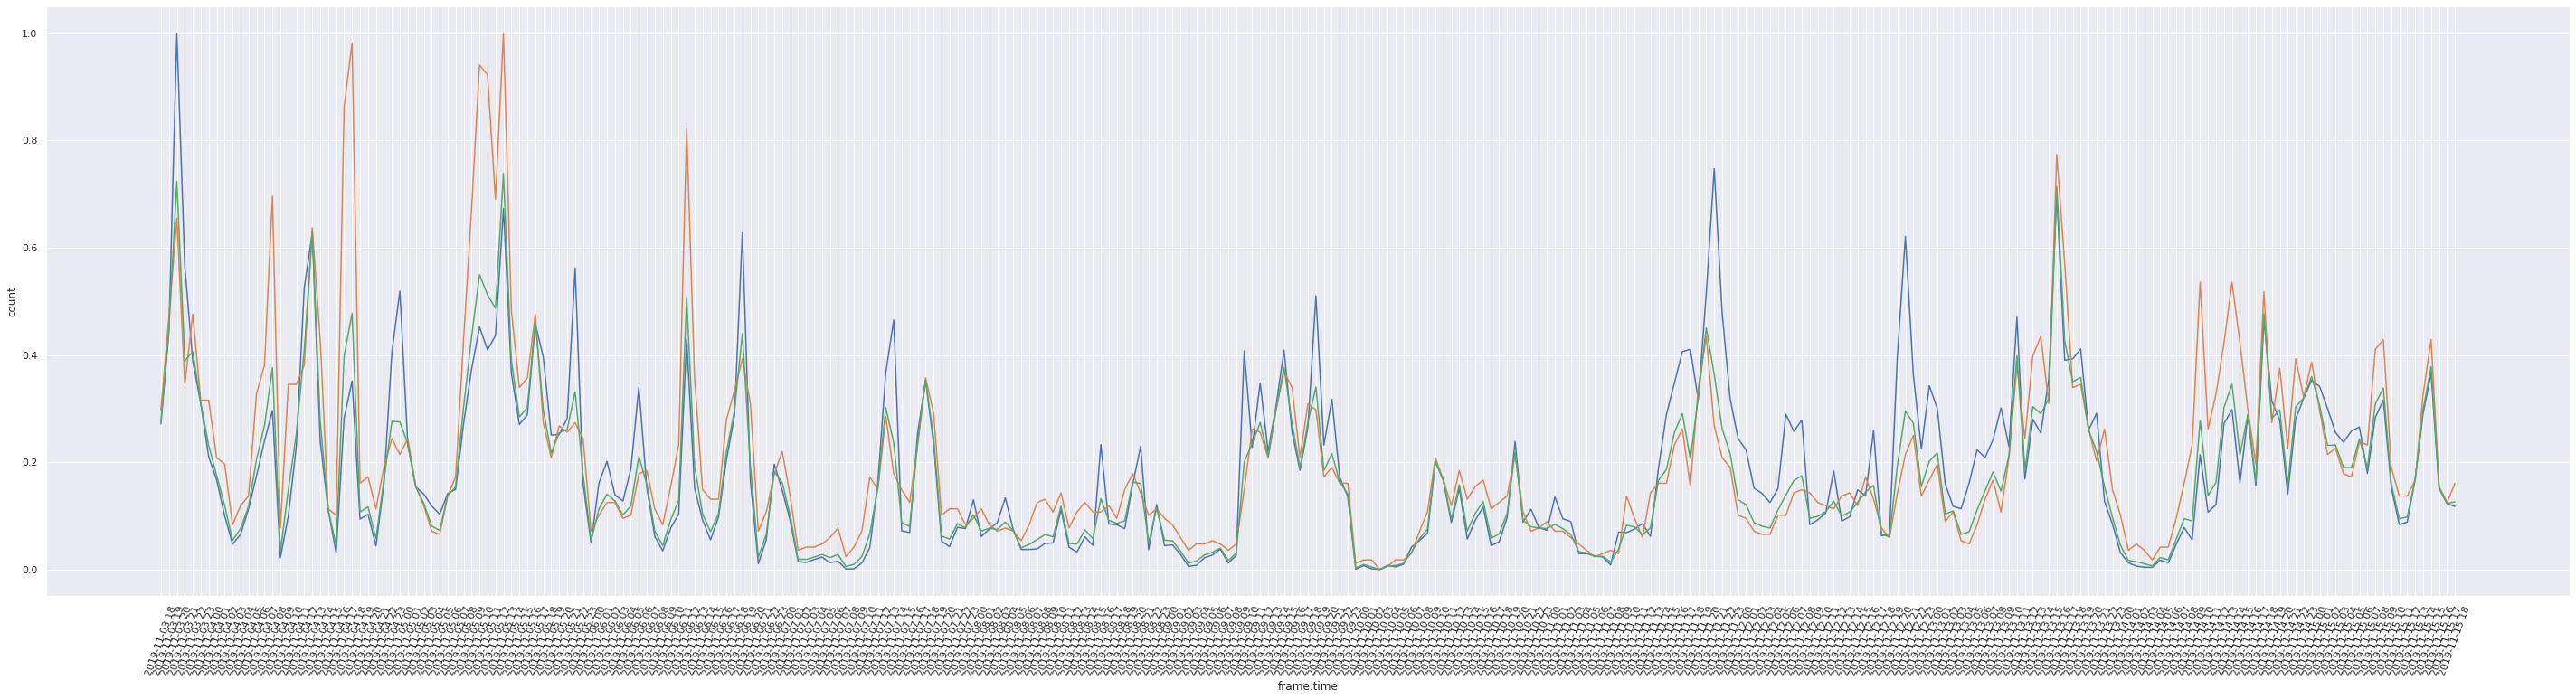
\includegraphics[width=\columnwidth]{report/final_report/images/crowedness.png}
    \captionof{figure}{Normalized data collected over the week. Orange is package count and blue is the MAC address count. Larger version of the same figure is available in Appendix B.}
    \label{fig:pandas_small}
    \medskip
\endgroup

\noindent Figure \ref{fig:pandas_small} represents the data collected over the week, with orange and blue being the normalized (0-1) package count and unique MAC address count. We see that given a few outliers, they follow a very similar trend, thus acting as relatively accurate indicators of crowdedness of a given space. Crowdedness was thus defined as a weighted average of the normalized values at a given hour, with a 80\% weight resting on the lower value, and a 20\% weight weight resting on the larger value. In cases where the two normalized values were very similar, this had little effect. On the other hand, in cases of large difference, this assumed that the larger value was an anomaly. For example, if a large group of people (great number of unique MAC addresses) enter a space but stay for a short amount of time, we do not want to include this in our dataset. Our definition of crowdedness hedges against this, as these unique MAC addresses would contribute a very small number of packages during their short stay. Referring back to Wang. et. al's work, this approach roughly accounts for their concern that visitors of short duration skew the forecast. 

% \noindent The first challenge that needs to be addressed is the identify people who just pass by the location or temporarily visit the location that is being monitored. This is important, otherwise there will be too much variation in the prediction and these predictions will not accurately represent the true crowdedness of the location being monitored. Based on the background research we have conducted, we realized that we can use Markov-based feedback  Recurrent Neural Networks (M-FRNN) to overcome the problem identifying people who are just passing by the location. The details of the model are explained under the "literature" subsection. Furthermore, we are going to use the signal strength and frequency information (data fields that start with \texttt{radiotap}) to filter signals that are coming from far locations that are outside of the monitored location. \\

% \noindent Additionally, we know about the maximum capacity of each location based on the architectural plans and we can use that number and the our predicted number to have a sense about crowdedness of the location that is being monitored. Furthermore, the Institute of Electrical and Electronics Engineers (IEEE) assigns specific MAC address prefixes to specific companies and they publish this data publicly. So, we can actually differentiate different devices based on their brands and understand if a device is a laptop or a mobile phone or a tablet or a watch. By using this information, we are going to fine tune the crowdedness prediction we generated by accounting the possibility of one person carrying multiple Wi-Fi devices.

\subsection{Data Analysis: Model Design and Justification}
\label{section:model_design}

\noindent Drawing inspiration from existing literature, we decided to use a recurrent neural network (RNN) as the backbone of our model. Specifically, we selected the Long short-term memory (LSTM) architecture for our package count and number of unique MAC address forecasting problems. LSTM cells were developed as a solution to the "vanishing gradient" \cite{lstm} problem that RNN models face: context remembrance across long time lags "takes a prohibitive amount of time or does not work at all" \cite{lstm}. LSTMs have additional gates (forget, input, and output gates) compared to traditional RNNs which allow for them to be more robust and aid the model in deciding whether certain values should be used or not. Essentially, the gates prevent values from being perturped by irrelevant input or noise \cite{lstm}. Moreover, stacking LSTM layers together allows for varied representations of the problem, often leading to better results, as was the case for our application. 


\newpage
\subsubsection{Version 1}
Initially, we began with two disconnected, stacked LSTM models. Meant to act as a feasibility check, we used these stacked LSTMs to independently forecast package count and unique MAC address count. This model was unsurprisingly discarded as the lack of connectedness did not produce a useful output, namely a crowdedness value. Nevertheless, this version was a key stepping stone in establishing the performance of the LSTMs forecasting capabilities. 

\begingroup
    \center
    \medskip
    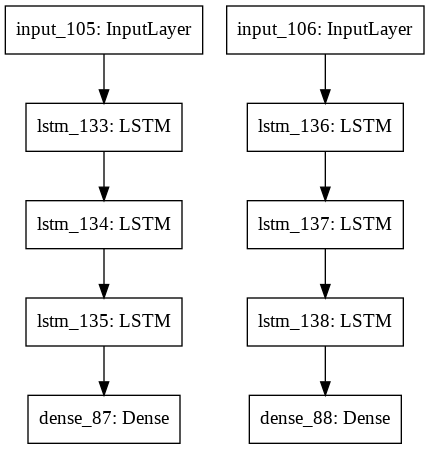
\includegraphics[width=0.9\columnwidth]{./images/v1_model.png}
    \captionof{figure}{Version 1 of the crowdedness forecasting model}
    \label{fig:v1}
    \medskip
\endgroup

\subsubsection{Version 2}
In an attempt to produce a unified value, we simply merged the two models by concatenating their output and feeding the merged output into a few dense layers. The model was trained with frame count and unique MAC address count as the X values and the corresponding crowdedness measure as the target value. While the model was able to pick up on trends after some tuning, we realized that the model was too much of a "blackbox" with too many enigmatic parameters to tune. Moreover, it seemed unnecessarily resource-heavy for the unimpressive output it was producing. Hence, we ultimately discarded this version as well. 


\begingroup
    \center
    \medskip
    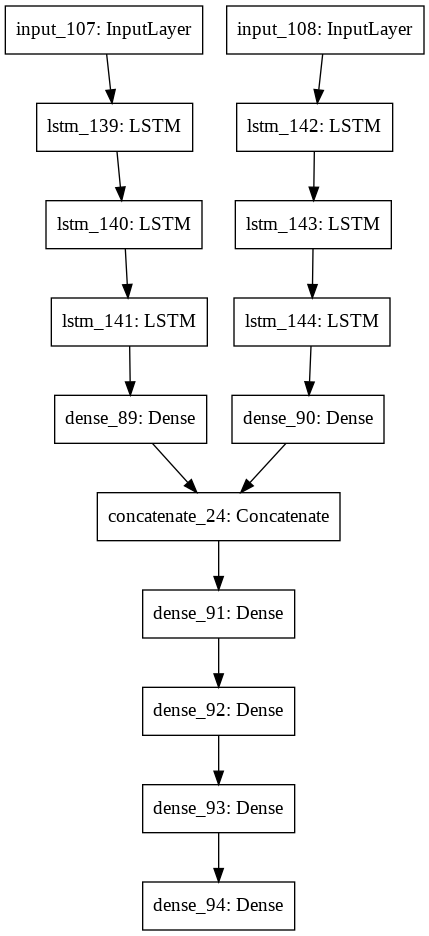
\includegraphics[width=0.9\columnwidth]{./images/v2_model.png}
    \captionof{figure}{Version 2 of the crowdedness forecasting model}
    \label{fig:v2}
    \medskip
\endgroup

\subsubsection{Version 3}
We finally settled on a modular approach that involved training models separately. In short, we split the version 2 model and encapsulated each section into its own model. We found this to be the best approach, as it allowed us to quickly recognize the weakest points in our model and target those layers specifically, instead of blinding tuning parameters. Figure \ref{fig:v3_expanded} (in Appendix C) shows the expanded model to provide a more detailed picture. 

\begingroup
    \center
    \medskip
    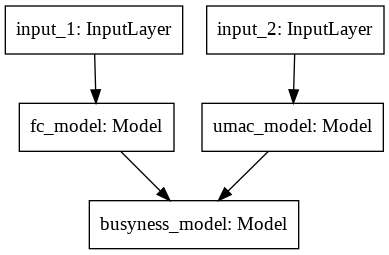
\includegraphics[width=\columnwidth]{./images/v3_model_high.png}
    \captionof{figure}{The final version of the crowdedness forecasting model at a higher level}
    \label{fig:v3}
    \medskip
\endgroup

\noindent Looking back at section \ref{section:data_engineering}, one may argue that our model could have been as simple as forecasting the crowdedness from the third dataset, which normalized the two input variables. While this simplification is recognized as a valid method, our model was developed under the assumption that package count data or the number of unique MAC addresses may want to be extracted from the model for other purposes. Had we simplified our model to operate on just normalized data, it would be extremely difficult to reverse the output and obtain these values. On the other hand, our final version implicitly calculates these and can be siphoned as an auxiliary output. 

\subsection{User Interface} 
\noindent The final step to our project was to have a simple, yet intuitive, user interface for presenting the forecasted data. To achieve this, we used the Bootstrap framework to design an aesthetic user interface and PHP to make it a dynamic web page capable of updating displayed data from the database. A SQLite database was be used to store the collected and processed data. The interface is available at \href{https://nyuad.app/flyway}{nyuad.app/flyway} website. The proposed and the implemented user interfaces can be seen in Figures \ref{fig:ui_proposed} and \ref{fig:ui_implemented}.\\

\begingroup
    \center
    \medskip
    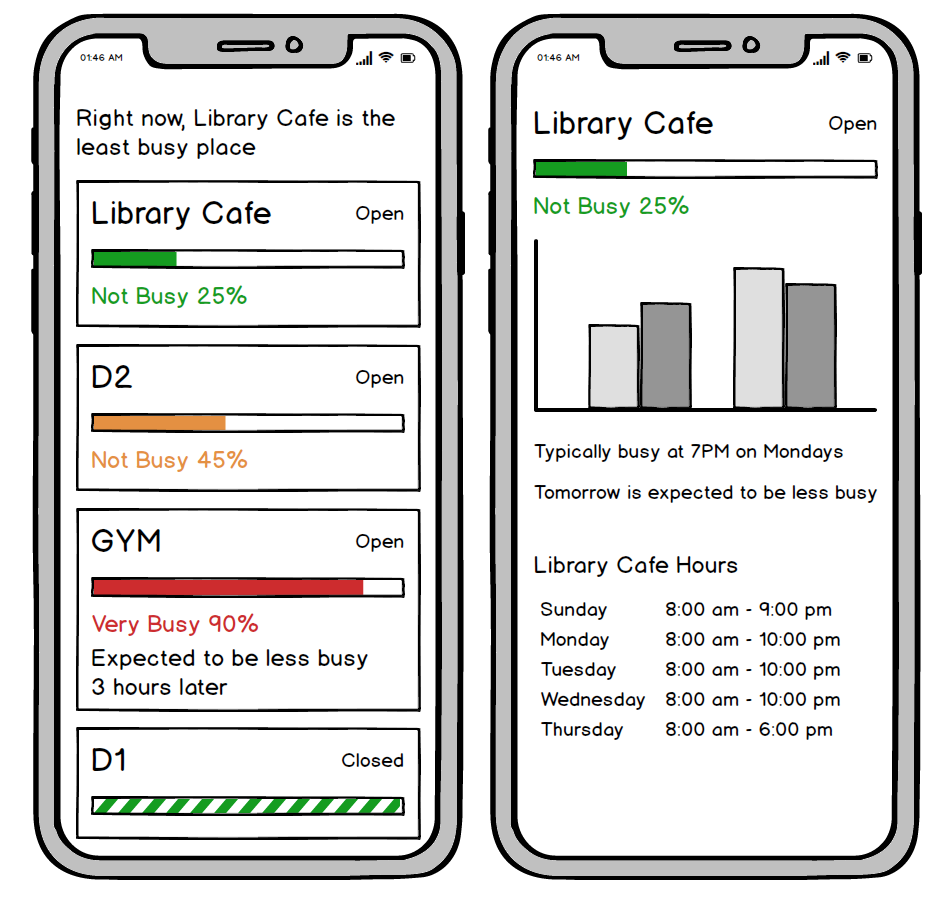
\includegraphics[width=0.9\columnwidth]{report/interim_report/images/ux.png}
    \captionof{figure}{Proposed user interface}
    \label{fig:ui_proposed}
    \medskip
\endgroup

\begingroup
    \center
    \medskip
    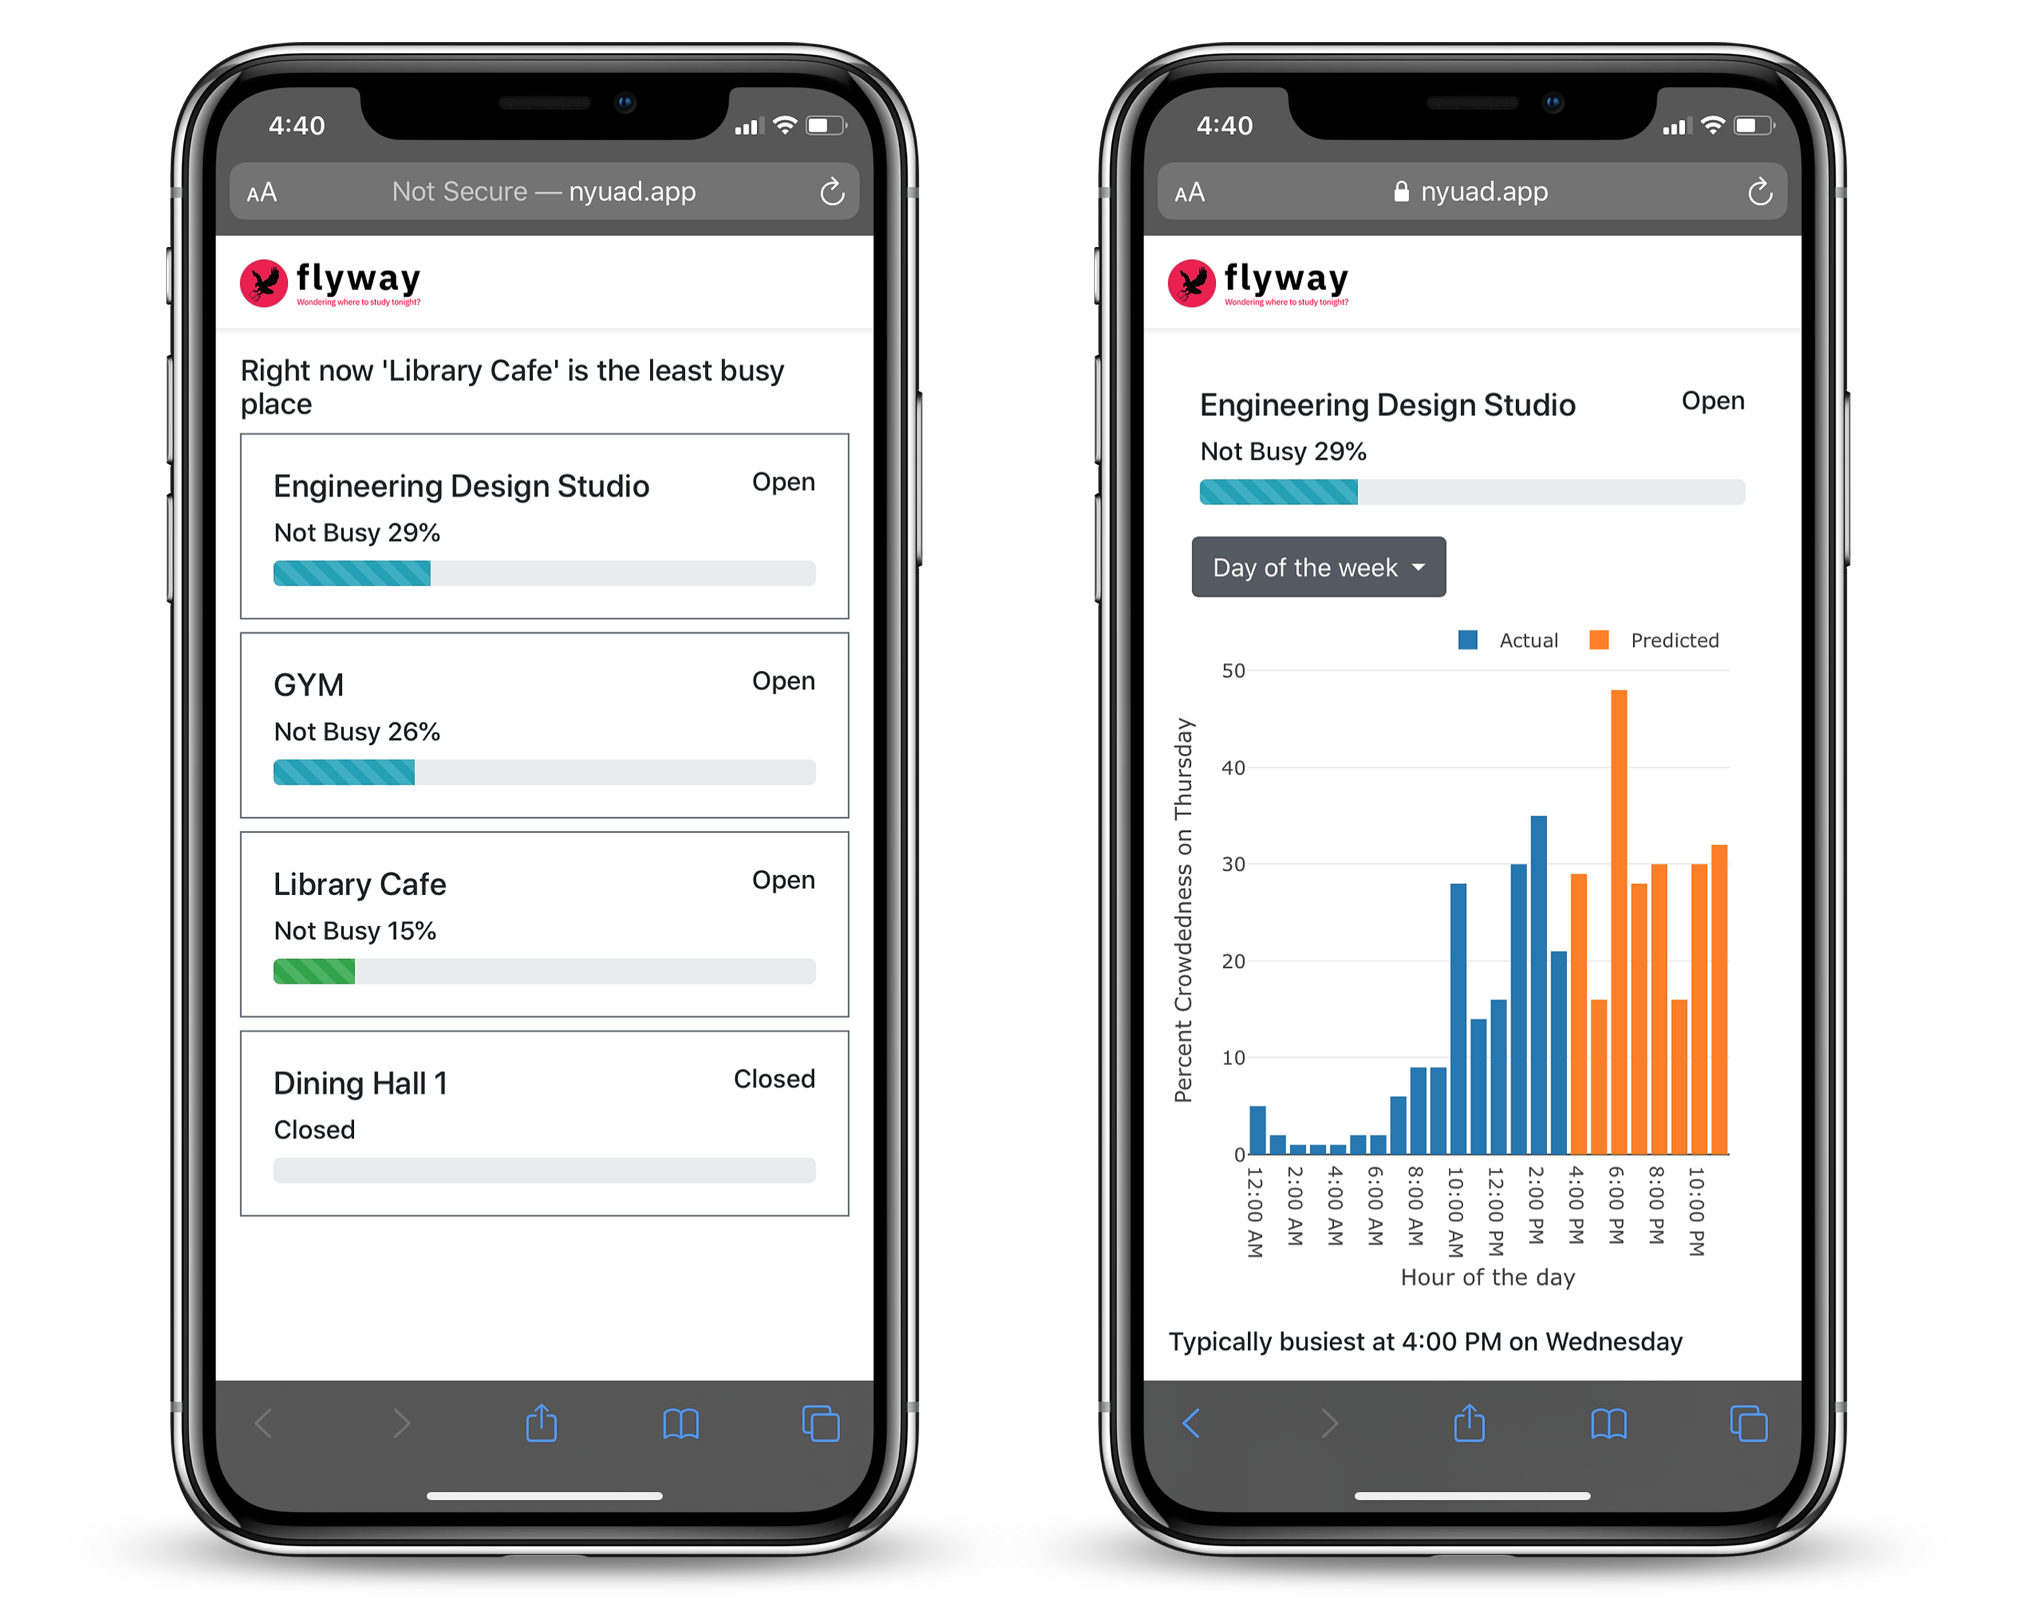
\includegraphics[width=\columnwidth]{report/final_report/images/ui_real_combined.png}
    \captionof{figure}{Implemented user interface, available at \href{https://nyuad.app/flyway}{nyuad.app/flyway}}
    \label{fig:ui_implemented}
    \medskip
\endgroup

\section{Results \& Analysis}

\noindent Looking at Figure \ref{fig:forecast} below, we found that our model performed quite well in capturing the general trends of the crowdedness factor. However, it seems to fail in capturing the larger spikes. This could partially be explained by the weight bias we fed into our crowdedness measurement. Perhaps, slightly adjusting the weight from the 80-20 split (favoring the lower crowdedness metric) could improve the model's ability to handle spikes. 

% very well able to capture the general trends

% difficulties in capturing the busiest season,due to the implicit bias in data

% slightly time shifted, can be corrected in the database

\begingroup
    \center
    \medskip
    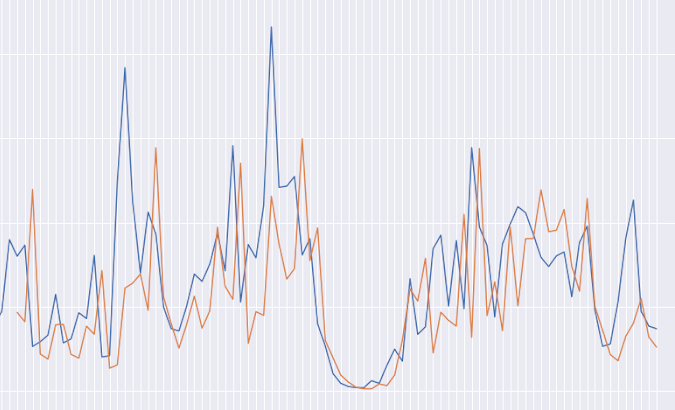
\includegraphics[width=\columnwidth]{report/final_report/images/forecasted.png}
    \captionof{figure}{Resulting crowdedness forecast. Blue line is the actual data, orange line is the predicted values.}
    \label{fig:forecast}
    \medskip
\endgroup


\noindent Given that the Keras model we compiled used the Mean-Squared Error (MSE) as a loss function, we were able to obtain the train and test MSE for our models, seen in the table below. 

\medskip
\begingroup
    \medskip
    \centering
    \def\arraystretch{1}
        \begin{tabular}{cc}
            \toprule
            Train MSE & Test MSE \\
            \midrule
            0.020 & 0.013\\
            \bottomrule
        \end{tabular}
    \captionof{table}{Mean squared error of our overall model}
    \label{table:fifty_runs}
    \medskip
\endgroup
\medskip

\noindent Since the difference between the Train and Test MSEs is quite insignificant, we are confident that our model was not any significant overfitting. \\

\begingroup
    \center
    \medskip
    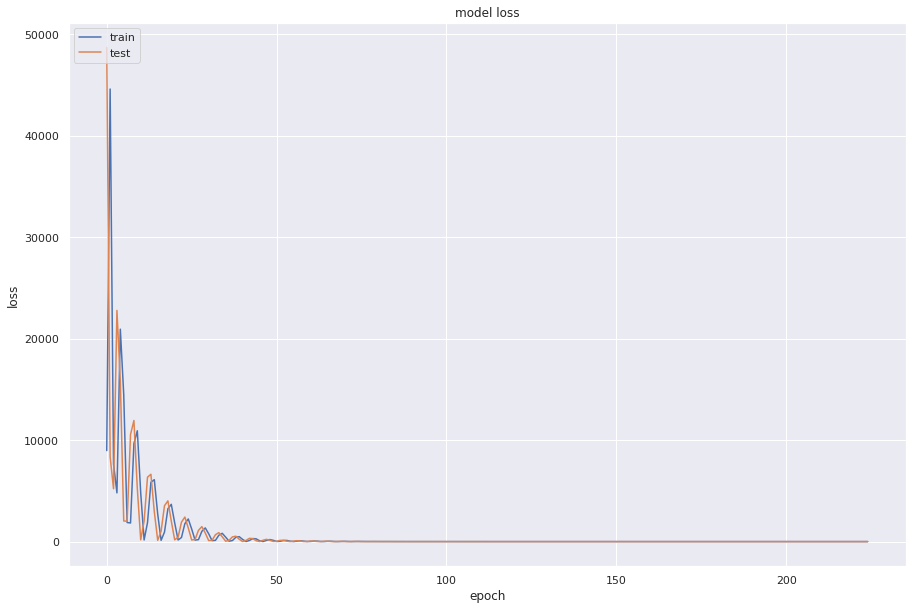
\includegraphics[width=\columnwidth]{report/final_report/images/crowdedness.png}
    \captionof{figure}{Train (blue) and test (orange losses for the crowdedness model}
    \label{fig:loss_crowdedness}
    \medskip
\endgroup

\noindent Due to our model having a modular design, we were able to analyze each of the components to determine where the poor performance was stemming from. Looking at the train/test MSE graph for the crowdedness dense network (see Figure \ref{fig:loss_crowdedness}), we see that the model performed fantastically. We also see that there was a relatively small gap between the train and test curves for the unique mac count LSTM model (see Figure \ref{fig:loss_mac}).

\begingroup
    \center
    \medskip
    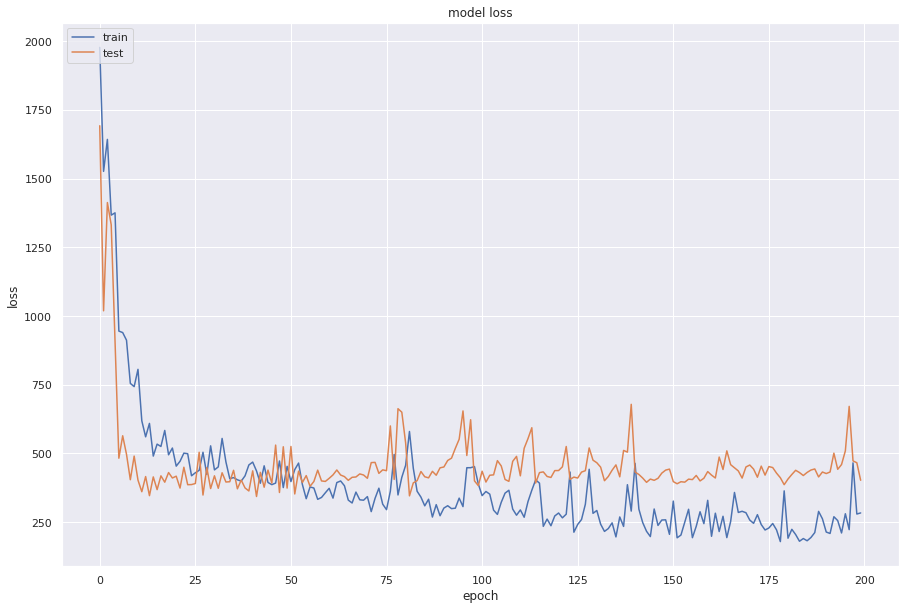
\includegraphics[width=\columnwidth]{report/final_report/images/macs.png}
    \captionof{figure}{Train (blue) and test (orange losses for the unique MAC count model}
    \label{fig:loss_mac}
    \medskip
\endgroup

Finally, we are able to infer that our weakest link was the package count LSTM model, as there is a significant and growing difference between the train and test curves as the number of epochs increases as shown in Figure \ref{fig:loss_fc}. Here our model was most likely overfitting to the training data. 

\begingroup
    \center
    \medskip
    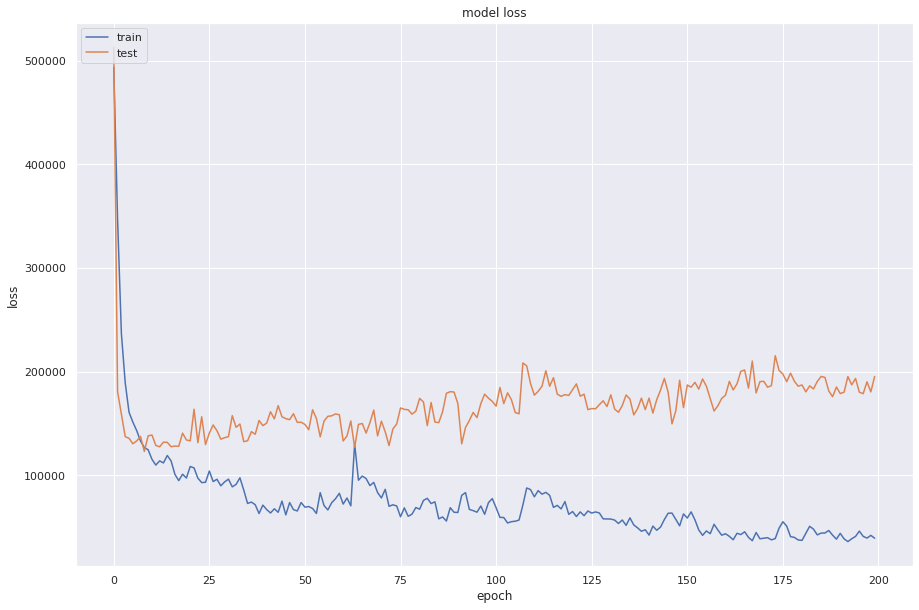
\includegraphics[width=\columnwidth]{report/final_report/images/frame_count.png}
    \captionof{figure}{Train (blue) and test (orange losses for the package count model}
    \label{fig:loss_fc}
    \medskip
\endgroup

\noindent Interestingly, this was the model where we supplemented the data with the one-hot encoded categorical data (day of the week and hour of the day) as shown in Figure \ref{fig:one_hot}. On the other hand, the unique MAC count LSTM model was simply provided the previous time-steps. It may be that combining categorical data along with continuous data deteriorated performance, or it may be that the categorical data was unneeded noise for the model.

\begingroup
    \center
    \medskip
    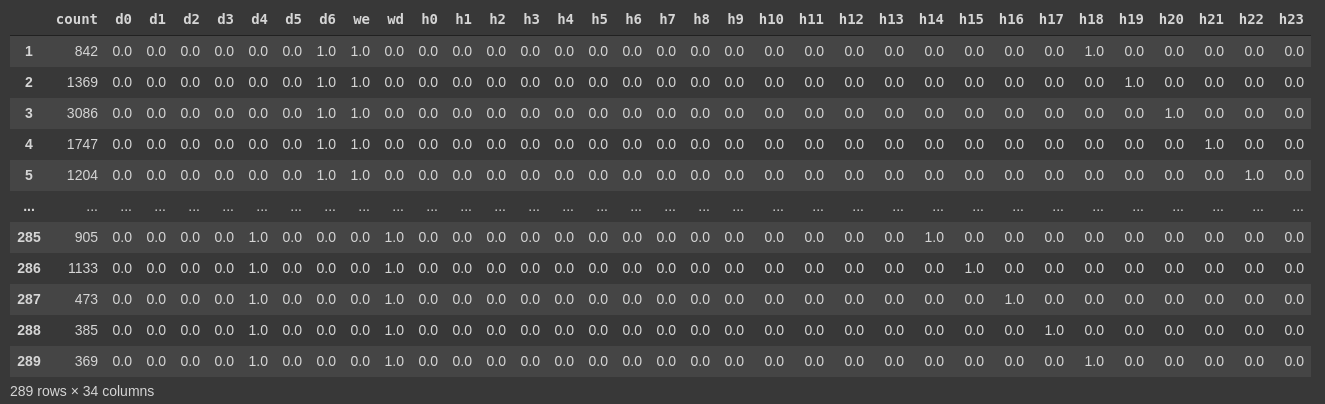
\includegraphics[width=\columnwidth]{report/final_report/images/one_hot.png}
    \captionof{figure}{Pandas dataframe preview of the one hot encoded data used for feeding the LSTM model}
    \label{fig:one_hot}
    \medskip
\endgroup

%%%%%%%%%%%%%%%%
%% Discussion %%
%%%%%%%%%%%%%%%%
% Yes, he wants separate conclusion and discussion
\section{Discussion} 





How networks work
Dealing with real life data collection
Choosing parameters carefully
Choosing to many variables decrease LSTM’s ability recognize features
Using frame count in addition to MAC addresses for making the prediction
Modularity within the project components
Models used are open to adding more features in the future



%%%%%%%%%%%%%%%%
%% Conclusion %%
%%%%%%%%%%%%%%%%
\section{Conclusion} 

\noindent The user interface, WiFi sensors, database, and the LSTM model all work together to provide a crowdedness forecast to the users. The data collected by the WiFi probes are stored in the database. The LSTM model periodically fetches the collected data and makes predictions, which are recorded into the database as well. Finally, the user interface has access to all of the past data and predictions. User interface shows all of these to the user in an elegant way.


> Future work
Adding validation option for users 
Cross checking results with actual people count in the spaces
Labelling
Deploying the data collectors in more areas on the campus
Extending the collected data types
Sound data
Co2 data
Camera maybe?
Improving the model and running the model directly on the data collection nodes for distributing the computation
Capturing a longer term data to capture more trends in the data



\printbibliography

\onecolumn 

\section{Appendix}

\subsection{Appendix A}
Here are the raw and the cleaned data. Note that y-scales are not same.

\begingroup
    \center
    \medskip
    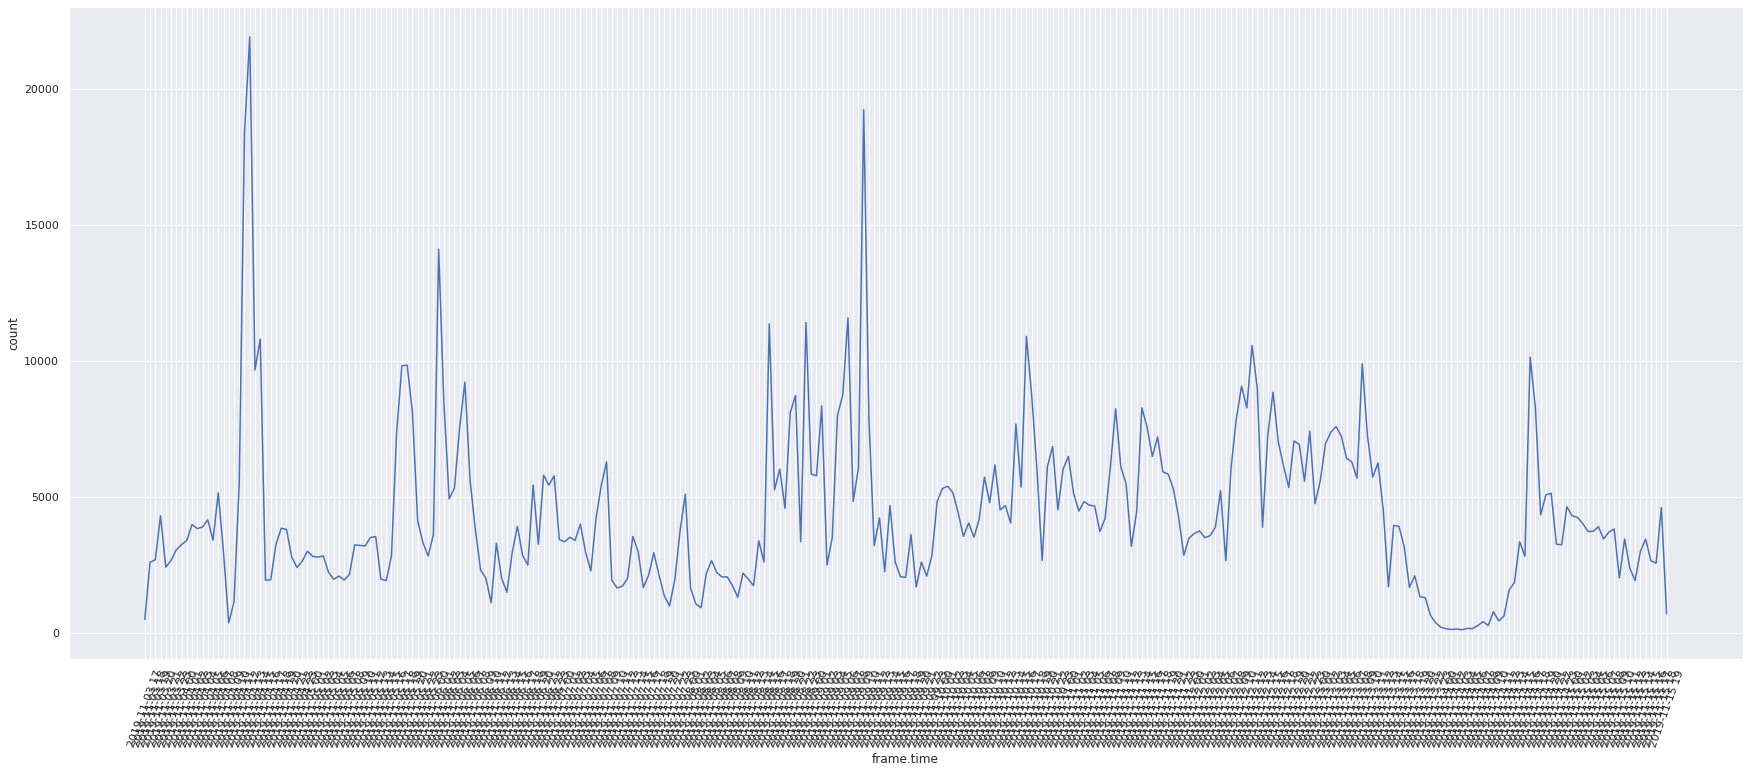
\includegraphics[width=\columnwidth]{report/final_report/images/not_celeaned.png}
    \captionof{figure}{Raw data before cleaning}
    \label{fig:raw}
    \medskip
\endgroup

\begingroup
    \center
    \medskip
    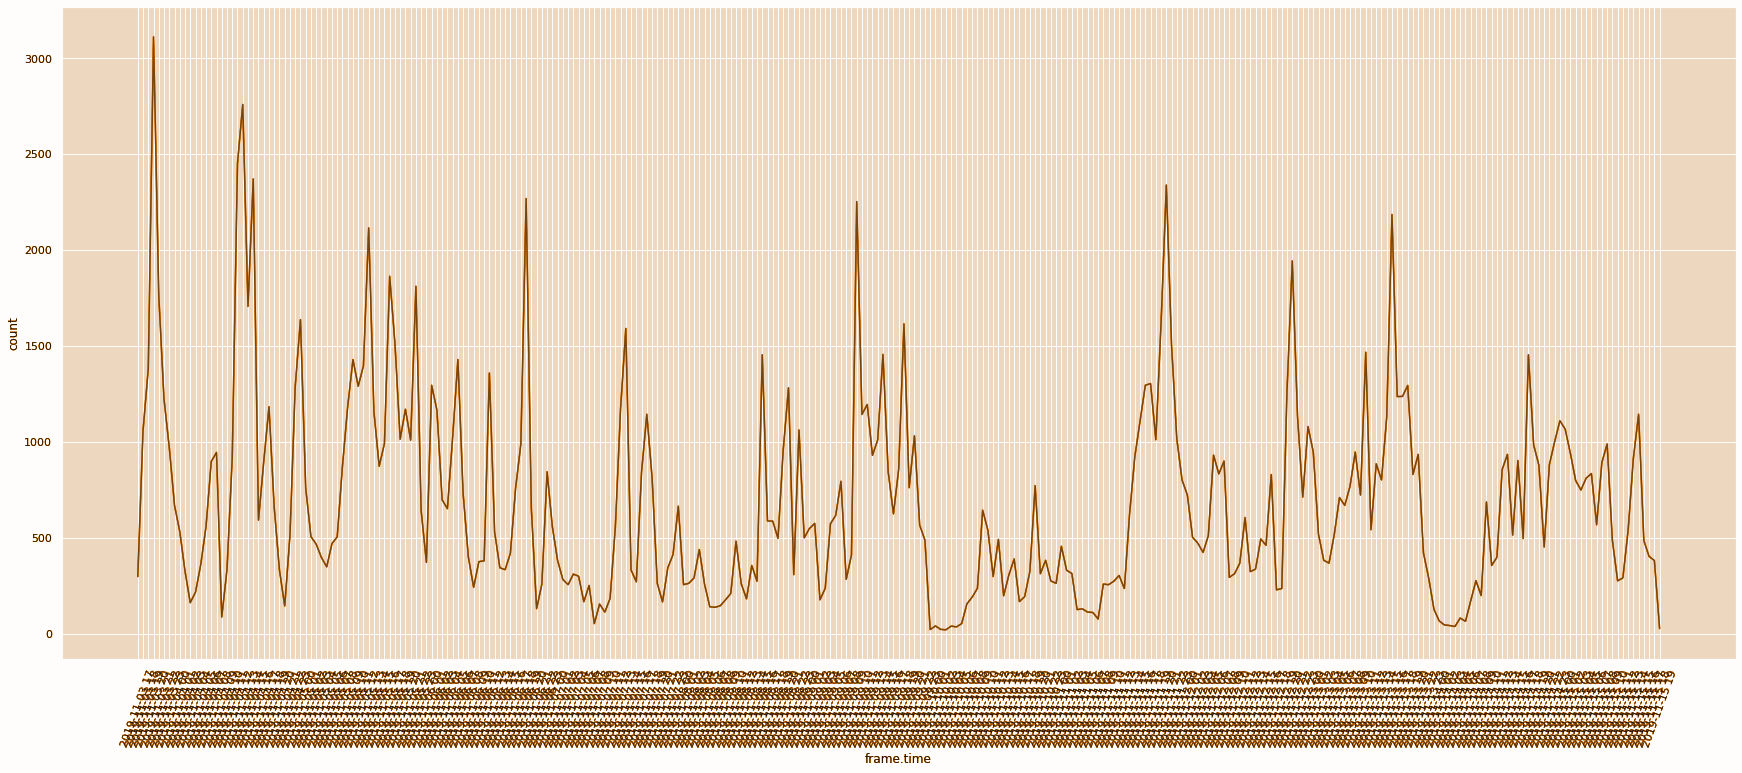
\includegraphics[width=\columnwidth]{report/final_report/images/cleaned.png}
    \captionof{figure}{Data after cleaning as explained in the data cleaning subsection}
    \label{fig:cleaned}
    \medskip
\endgroup

\subsection{Appendix B}

\begingroup
    \center
    \medskip
    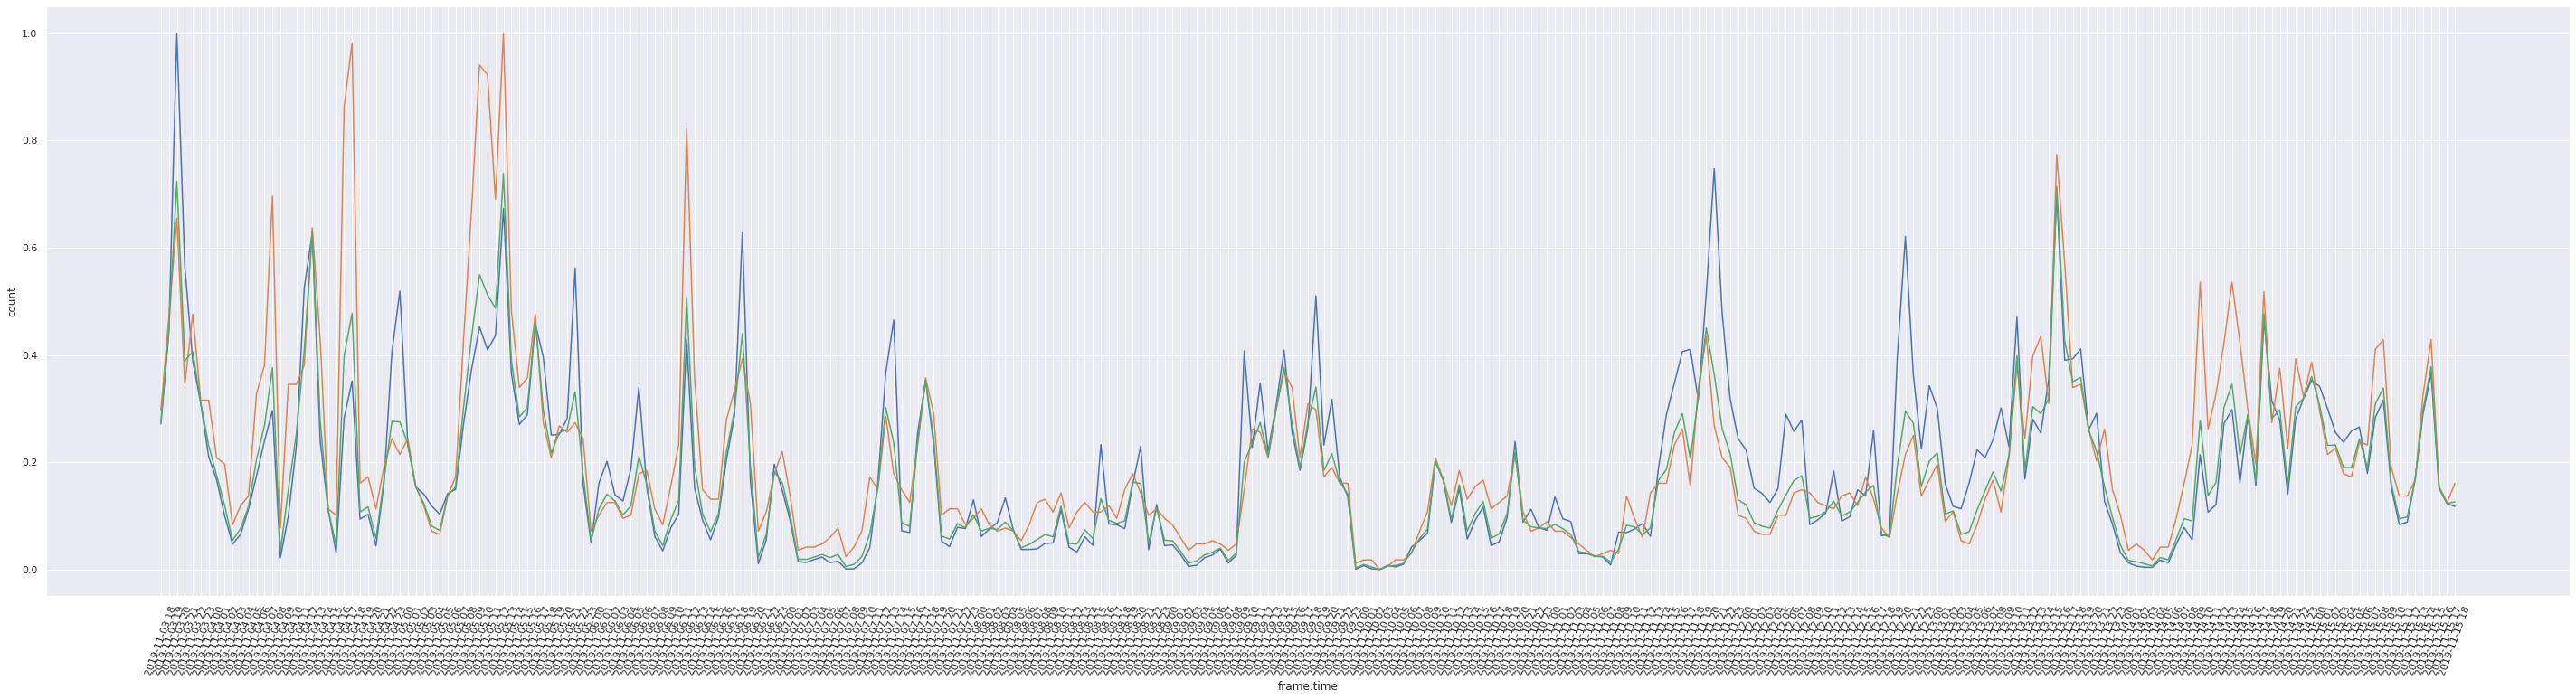
\includegraphics[width=\columnwidth]{report/final_report/images/crowedness.png}
    \captionof{figure}{Orange and blue represent the normalized package count and unique addresses data, respectively. Green represents crowdedness.}
    \label{fig:pandas}
    \medskip
\endgroup


\subsection{Appendix C}

\begingroup
    \center
    \medskip
    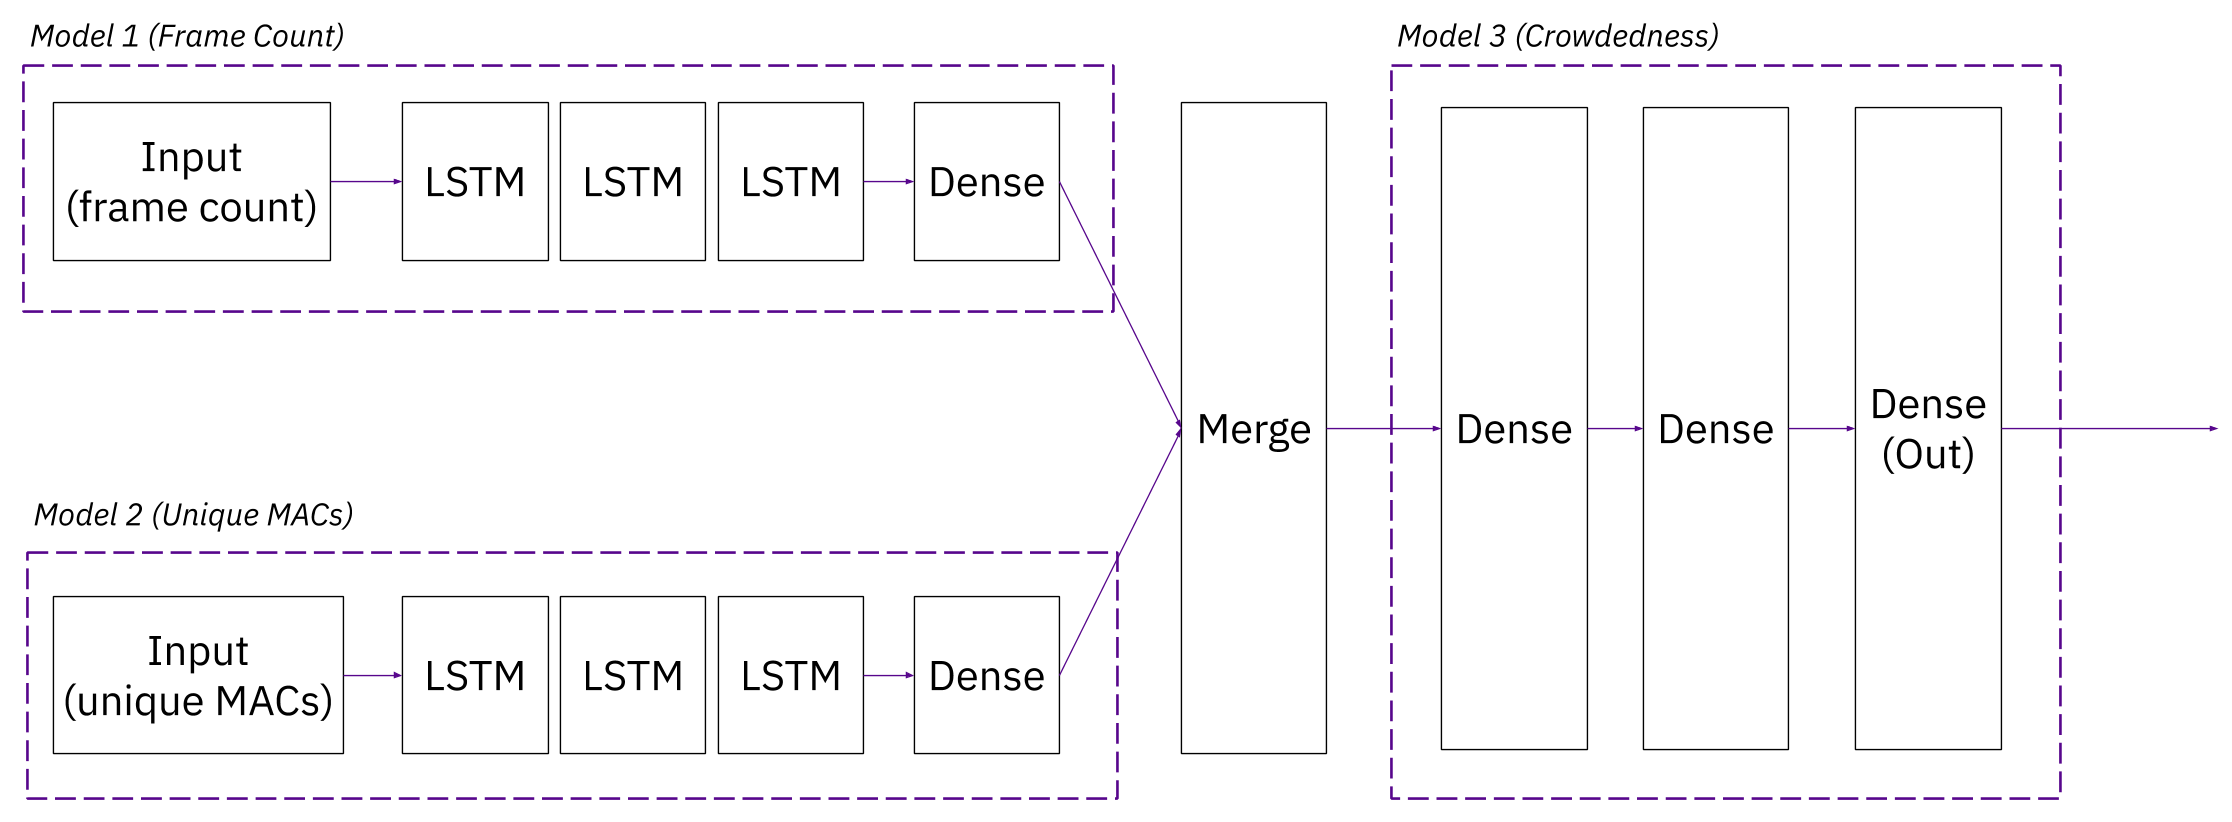
\includegraphics[width=\columnwidth]{./images/v3_model.png}
    \captionof{figure}{The final version of the crowdedness forecasting model expanded}
    \label{fig:v3_expanded}
    \medskip
\endgroup

\end{document}

%%%%%%%%%%%%%%%
%% Equations %%
%%%%%%%%%%%%%%%

% \begin{equation}
%     \begin{split}
%         X &\texttt{\char`\~} Poisson(\lambda) \\
%         \\
%         P(X=k) &= \frac{\lambda^k e^{-\lambda}}{k!} \\
%         \\
%         \EX(k) &= e^{-\lambda}\sum_{k=1}^{\infty} \frac{\lambda^n}{(n-1)!}\\
%         \\
%         &= e^{-\lambda}\lambda\sum_{k=1}^{\infty} \frac{\lambda^{k-1}}{(k-1)!}\\
%         \\
%         &= e^{-\lambda}\lambda\sum_{n=0}^{\infty} \frac{\lambda^{n}}{(n)!}\\
%         \\
%         &= e^{-\lambda}\lambda e^{\lambda} = \lambda\\
%     \end{split}
%     \label{eq:mutual}
% \end{equation}


% \begin{equation}
%     \begin{split}
%         \lambda = \frac{\sum_{i=1}^{n}D_i}{n}
%     \end{split}
%     \label{eq:poisson_distribution}
% \end{equation}

%%%%%%%%%%%
%% Table %%
%%%%%%%%%%%

% \begingroup
%     \medskip
%     \centering
%     \def\arraystretch{1.5}
%         \begin{tabular}{lcc}
%             \toprule
%             & Random Network & Scale-Free Network \\
%             \midrule
%             Avg. of Avg. Degree    & 3.9988    &  4.0035   \\
%             Var. of Avg. Degree    & 7.6800$\times 10^{-7}$ & 3.1156$\times 10^{-6}$  \\
%             Avg. of Avg. Distance  & 5.5694 & 5.0935    \\
%             Var. of Avg. Distance  & 1.5507 & 0.5377   \\
%             \bottomrule
%         \end{tabular}
%     \captionof{table}{Statistics of fifty runs where \\ n = 5,000, e = 10,000}
%     \label{table:fifty_runs}
%     \medskip
% \endgroup
